Para la validación del prototipo se emplean los mismos bancos de prueba mencionados en la Sección (\ref{sec:PlanValidacion}), ya que no existe una diferencia sustancial que implique la necesidad de alterar dichos ensayos.

\Subsection{Validación pruebas funcionales}

Las validaciones a continuación están relacionadas a aspectos funcionales de los sensores.
Comenzaremos con el periodo de muestreo de estos como indica \textit{T-INT-FUN-07}
\begin{figure}[H]
	\centering
    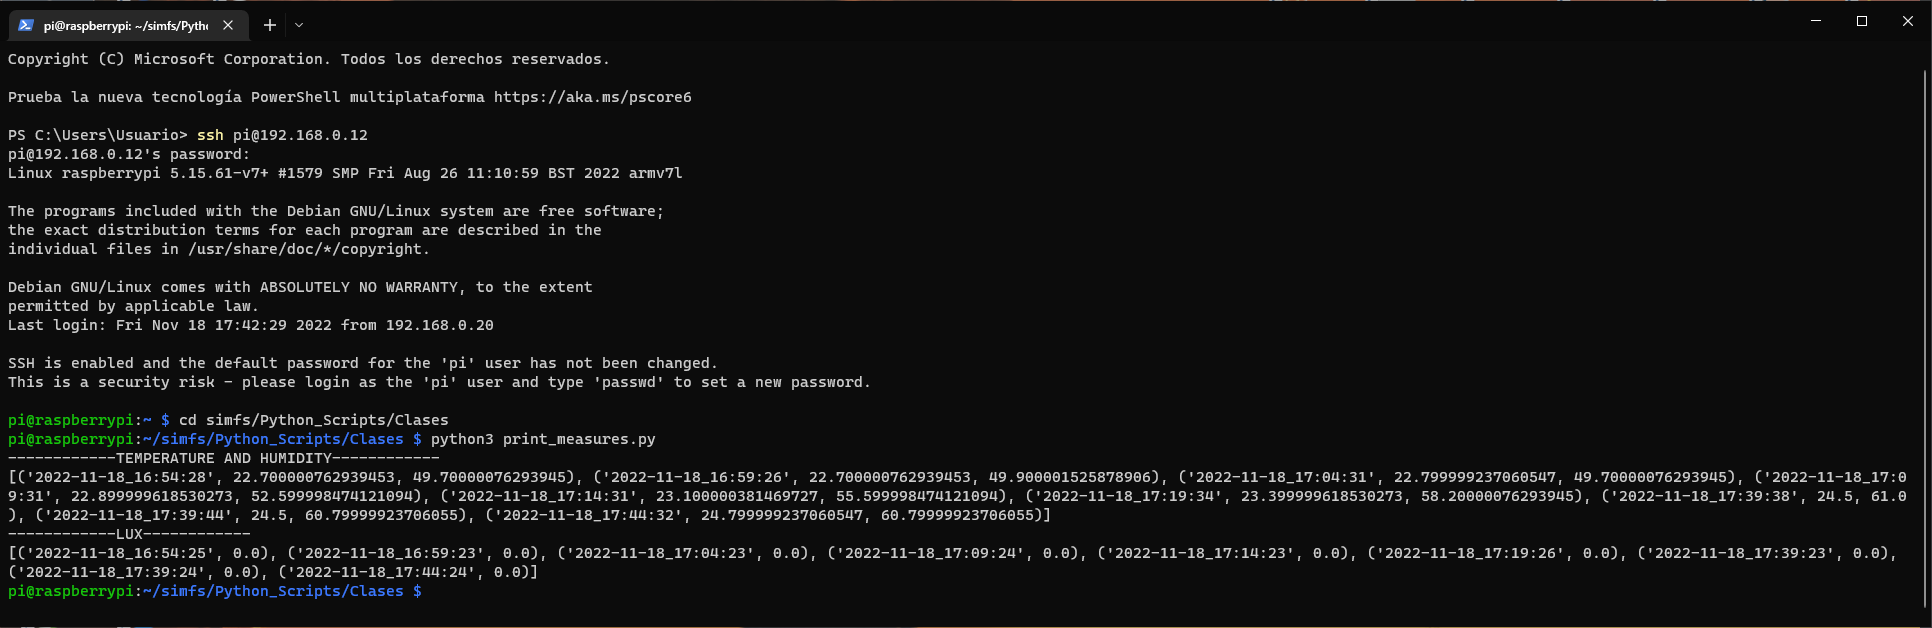
\includegraphics[width=1\linewidth]{ImagenesValidacion del prototipo/T-INT-FUN-07}
	\caption{Validación de funcionalidad \textit{T-INT-FUN-07}.}
\end{figure}

Se puede corroborar que las mediciones son cada 5 minutos. Luego se realizan las pruebas acordes a \textit{T-INT-FUN-08}.
\begin{figure}[H]
	\centering
    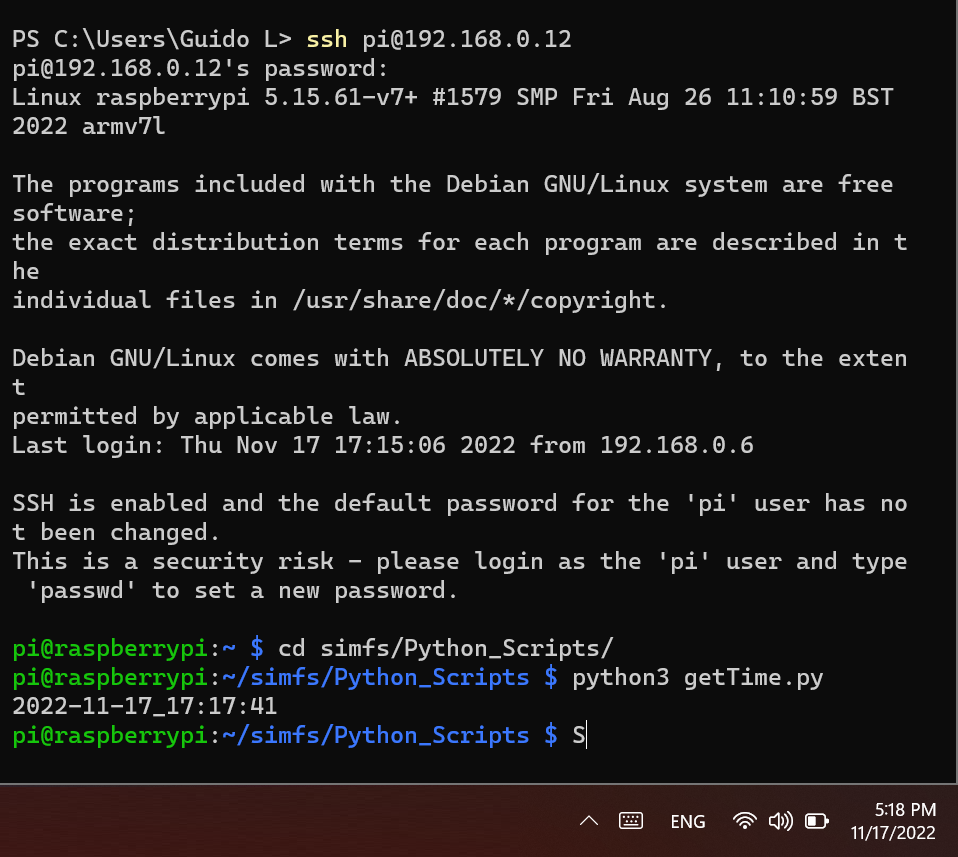
\includegraphics[width=0.8\linewidth]{ImagenesValidacion del prototipo/TINTFUN8}
	\caption{Validación de funcionalidad \textit{T-INT-FUN-08}.}
\end{figure}


Las siguientes validaciones están relacionadas con el manejo apropiado del tiempo, en particular la siguiente corresponde a \textit{T-INT-FUN-08}.
\begin{figure}[H]
	\centering
    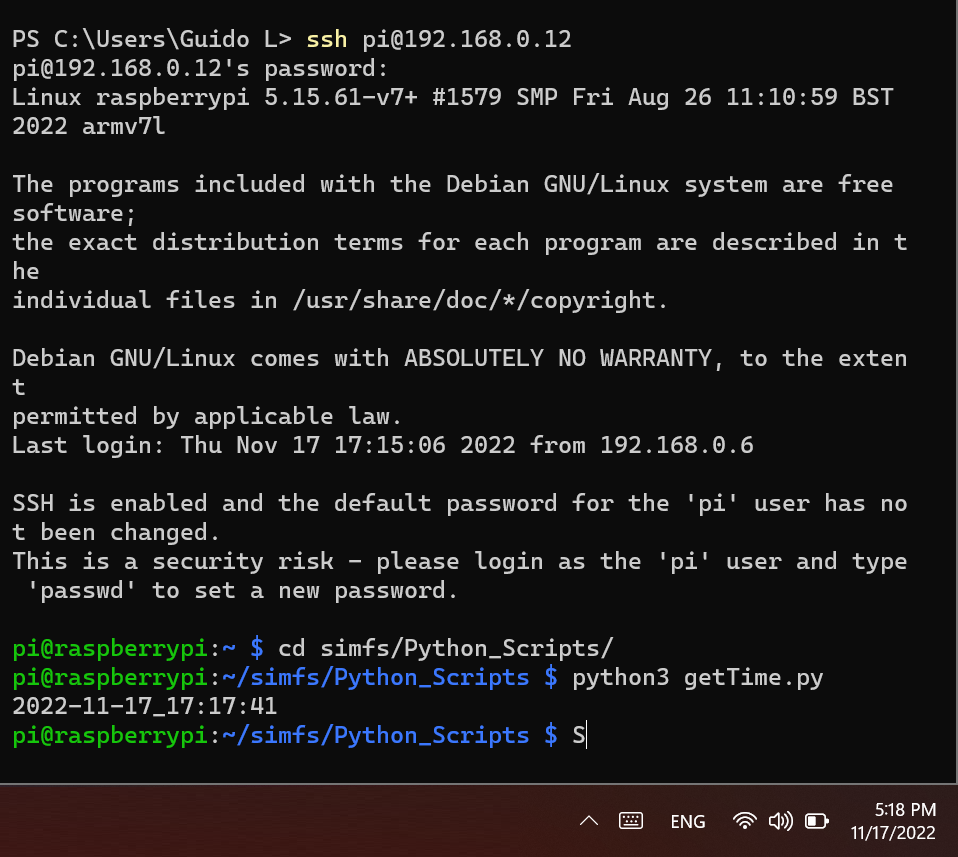
\includegraphics[width=0.8\linewidth]{ImagenesValidacion del prototipo/TINTFUN8}
	\caption{Validación de funcionalidad \textit{T-INT-FUN-08}.}
\end{figure}

Se observa que ambos tiempos coinciden, por lo que se considera que la prueba concluyó de manera exitosa. De manera similar se dio con la prueba \textit{T-INT-FUN-6}, donde se varió la posición del módulo BLE, observando los cambios de su presencia.
\begin{figure}[H]
	\centering
		\begin{subfigure}{0.49\textwidth}
			\centering
			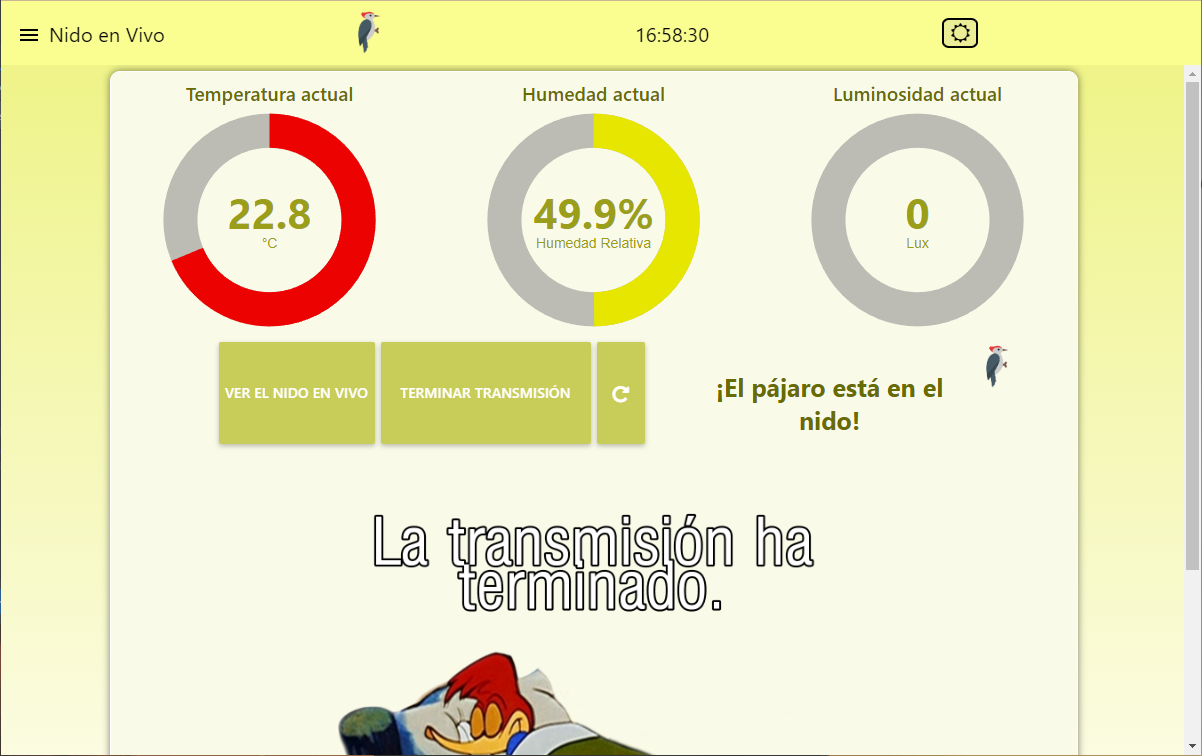
\includegraphics[width=\linewidth]{ImagenesValidacion del prototipo/T-INT-FUN-6-1}		
			\caption{\quotes{El pájaro está en el nido}.}
		\end{subfigure}\hfill
		\begin{subfigure}{0.49\textwidth}
			\centering
			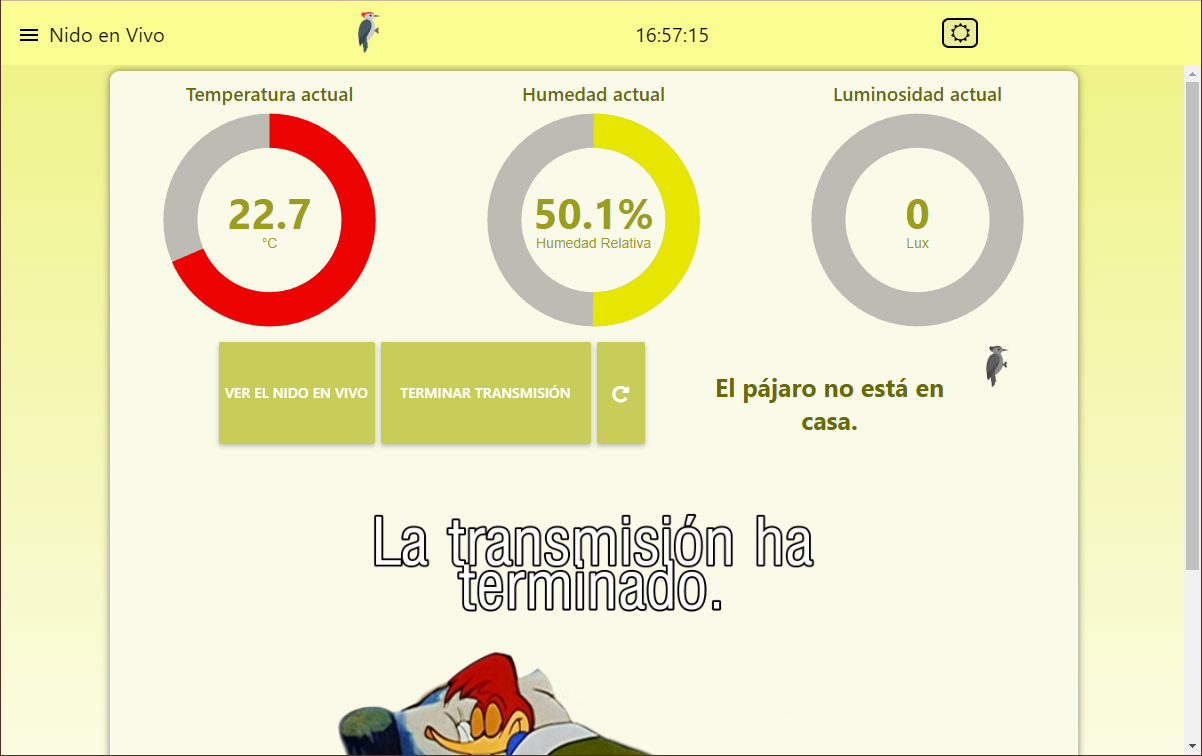
\includegraphics[width=\linewidth]{ImagenesValidacion del prototipo/T-INT-FUN-6-2}
			\caption{\quotes{El pájaro no está en casa}.}
		\end{subfigure}
	\caption{Validación de funcionalidad \textit{T-INT-FUN-6}.}
\end{figure}
\begin{figure}[H]
\centering
	\begin{subfigure}{0.49\textwidth}
		\centering
		\includegraphics[width=\linewidth]{ImagenesValidacion del prototipo/T-INT-FUN11a}	
		\caption{Beacon fuera del nido.}
	\end{subfigure}\hfill
	\begin{subfigure}{0.49\textwidth}
		\centering
		\includegraphics[width=\linewidth]{ImagenesValidacion del prototipo/T-INT-FUN11b}
		\caption{Beacon en el nido.}
	\end{subfigure}
\end{figure}
La siguiente prueba corresponde a \textit{T-INT-FUN-09}. En esta se desenergiza la \rspi, y luego de esperar el tiempo apropiado, se la energiza nuevamente corroborando que la hora correspondiente al módulo RTC sea correcta.
\begin{figure}[H]
\centering
	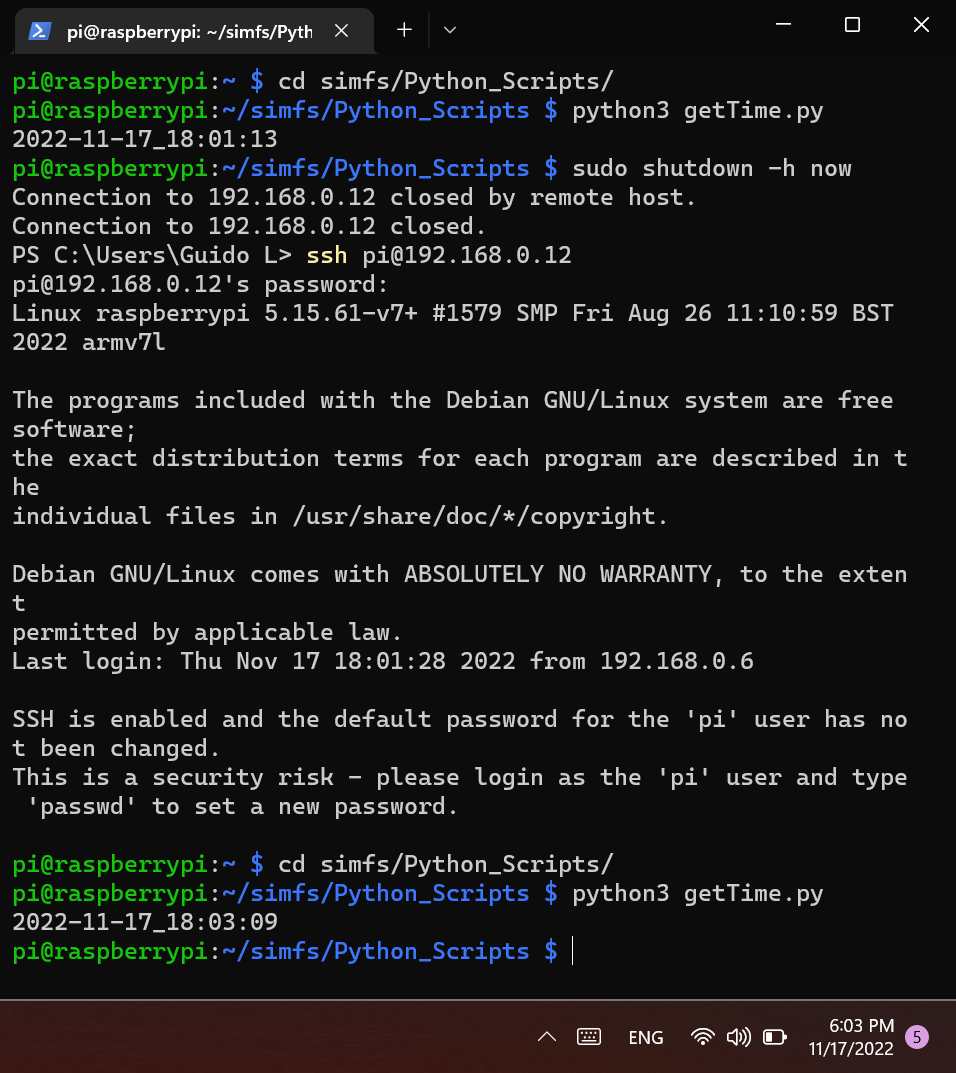
\includegraphics[width=0.8\linewidth]{ImagenesValidacion del prototipo/TINTFUN9}
	\caption{Validación de funcionalidad \textit{T-INT-FUN-09}.}
\end{figure}

El test \textit{T-INT-FUN-05} se concluyó de manera satisfactoria. Resultados similares a los obtenidos se encuentran presentes en la Figura (\ref{fig:foto_camara_filtro}), donde se comparan fotos similares con y sin filtro.

Disponiendo del banco de pruebas \#3, se corroboró mediante observación los tests de funcionalidad \textit{T-INT-FUN-04} y \textit{T-INT-FUN-12}. Se garantizó que la imagen mostrada al usuario sea la adecuada y que se vea de manera fidedigna, es decir que la transmisión sea de calidad y fluida.
\begin{figure}[H]
	\centering
    	\begin{subfigure}{0.49\textwidth}
        	\centering
        	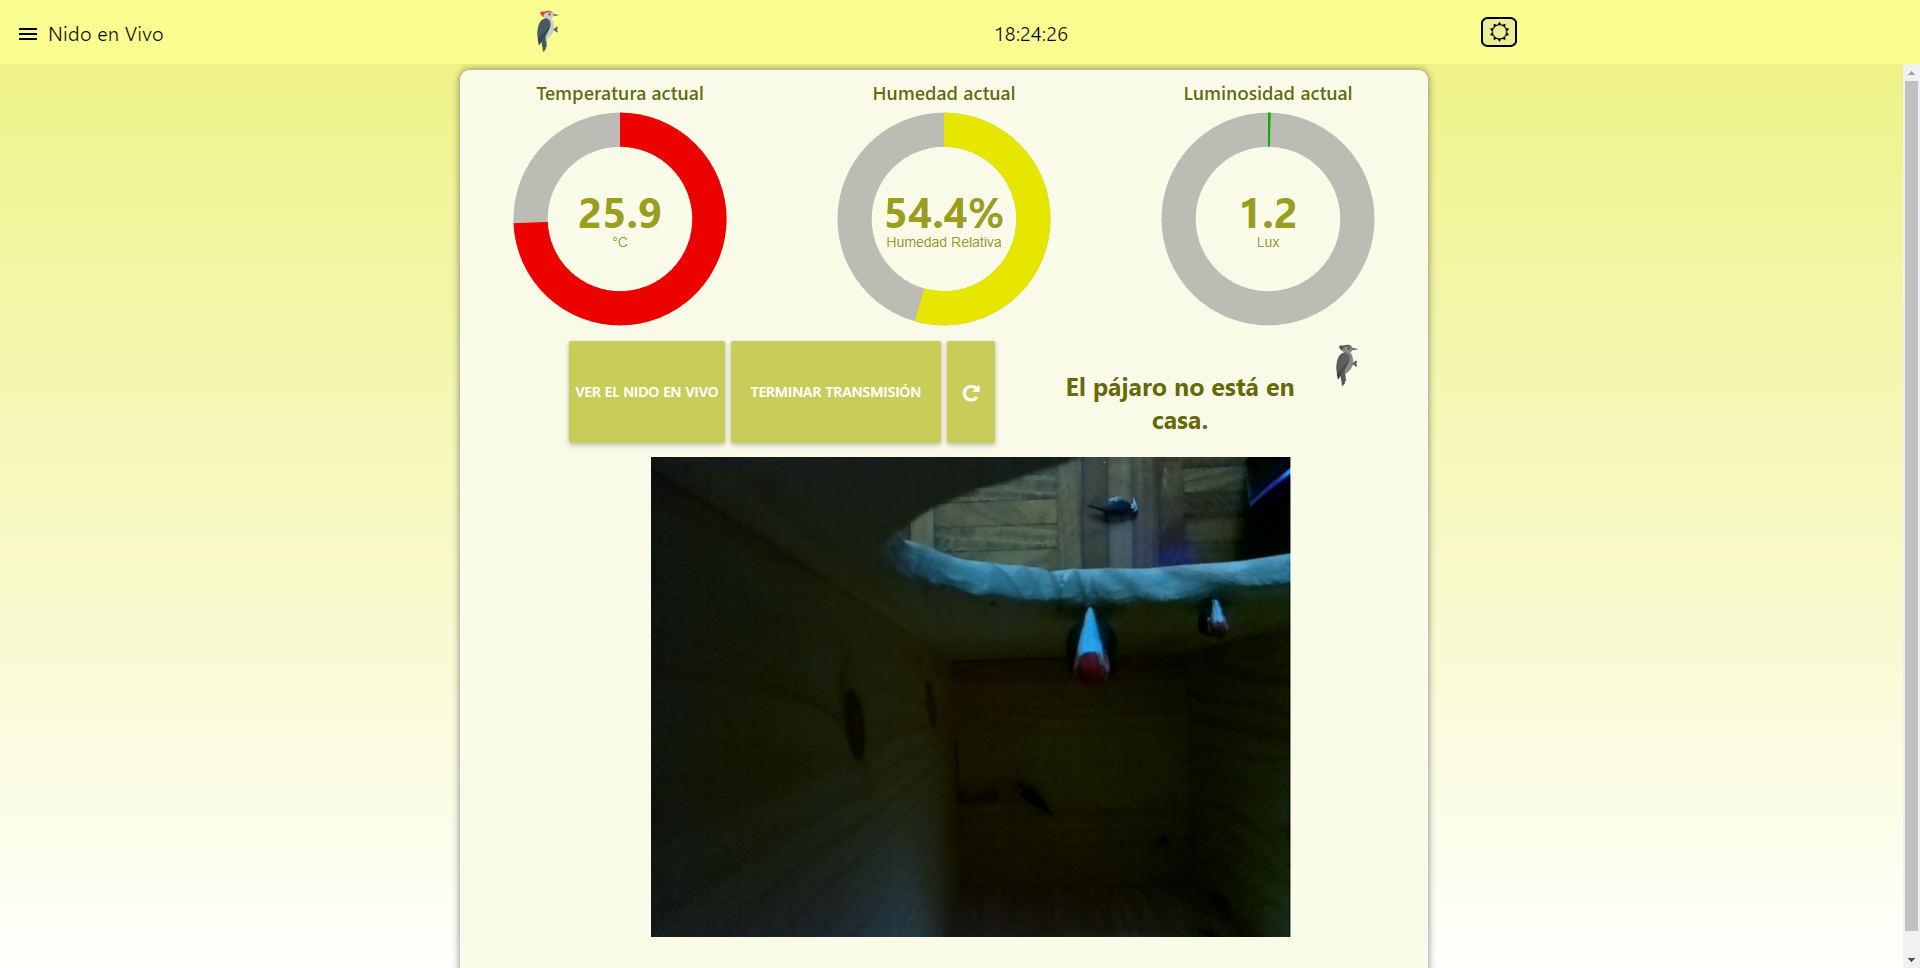
\includegraphics[width=\linewidth]{ImagenesValidacion del prototipo/t-int-fun-04-12-1}		
			\caption{Vista de la transmisión en vivo del nido.}
        \end{subfigure}\hfill
        \begin{subfigure}{0.49\textwidth}
        	\centering
        	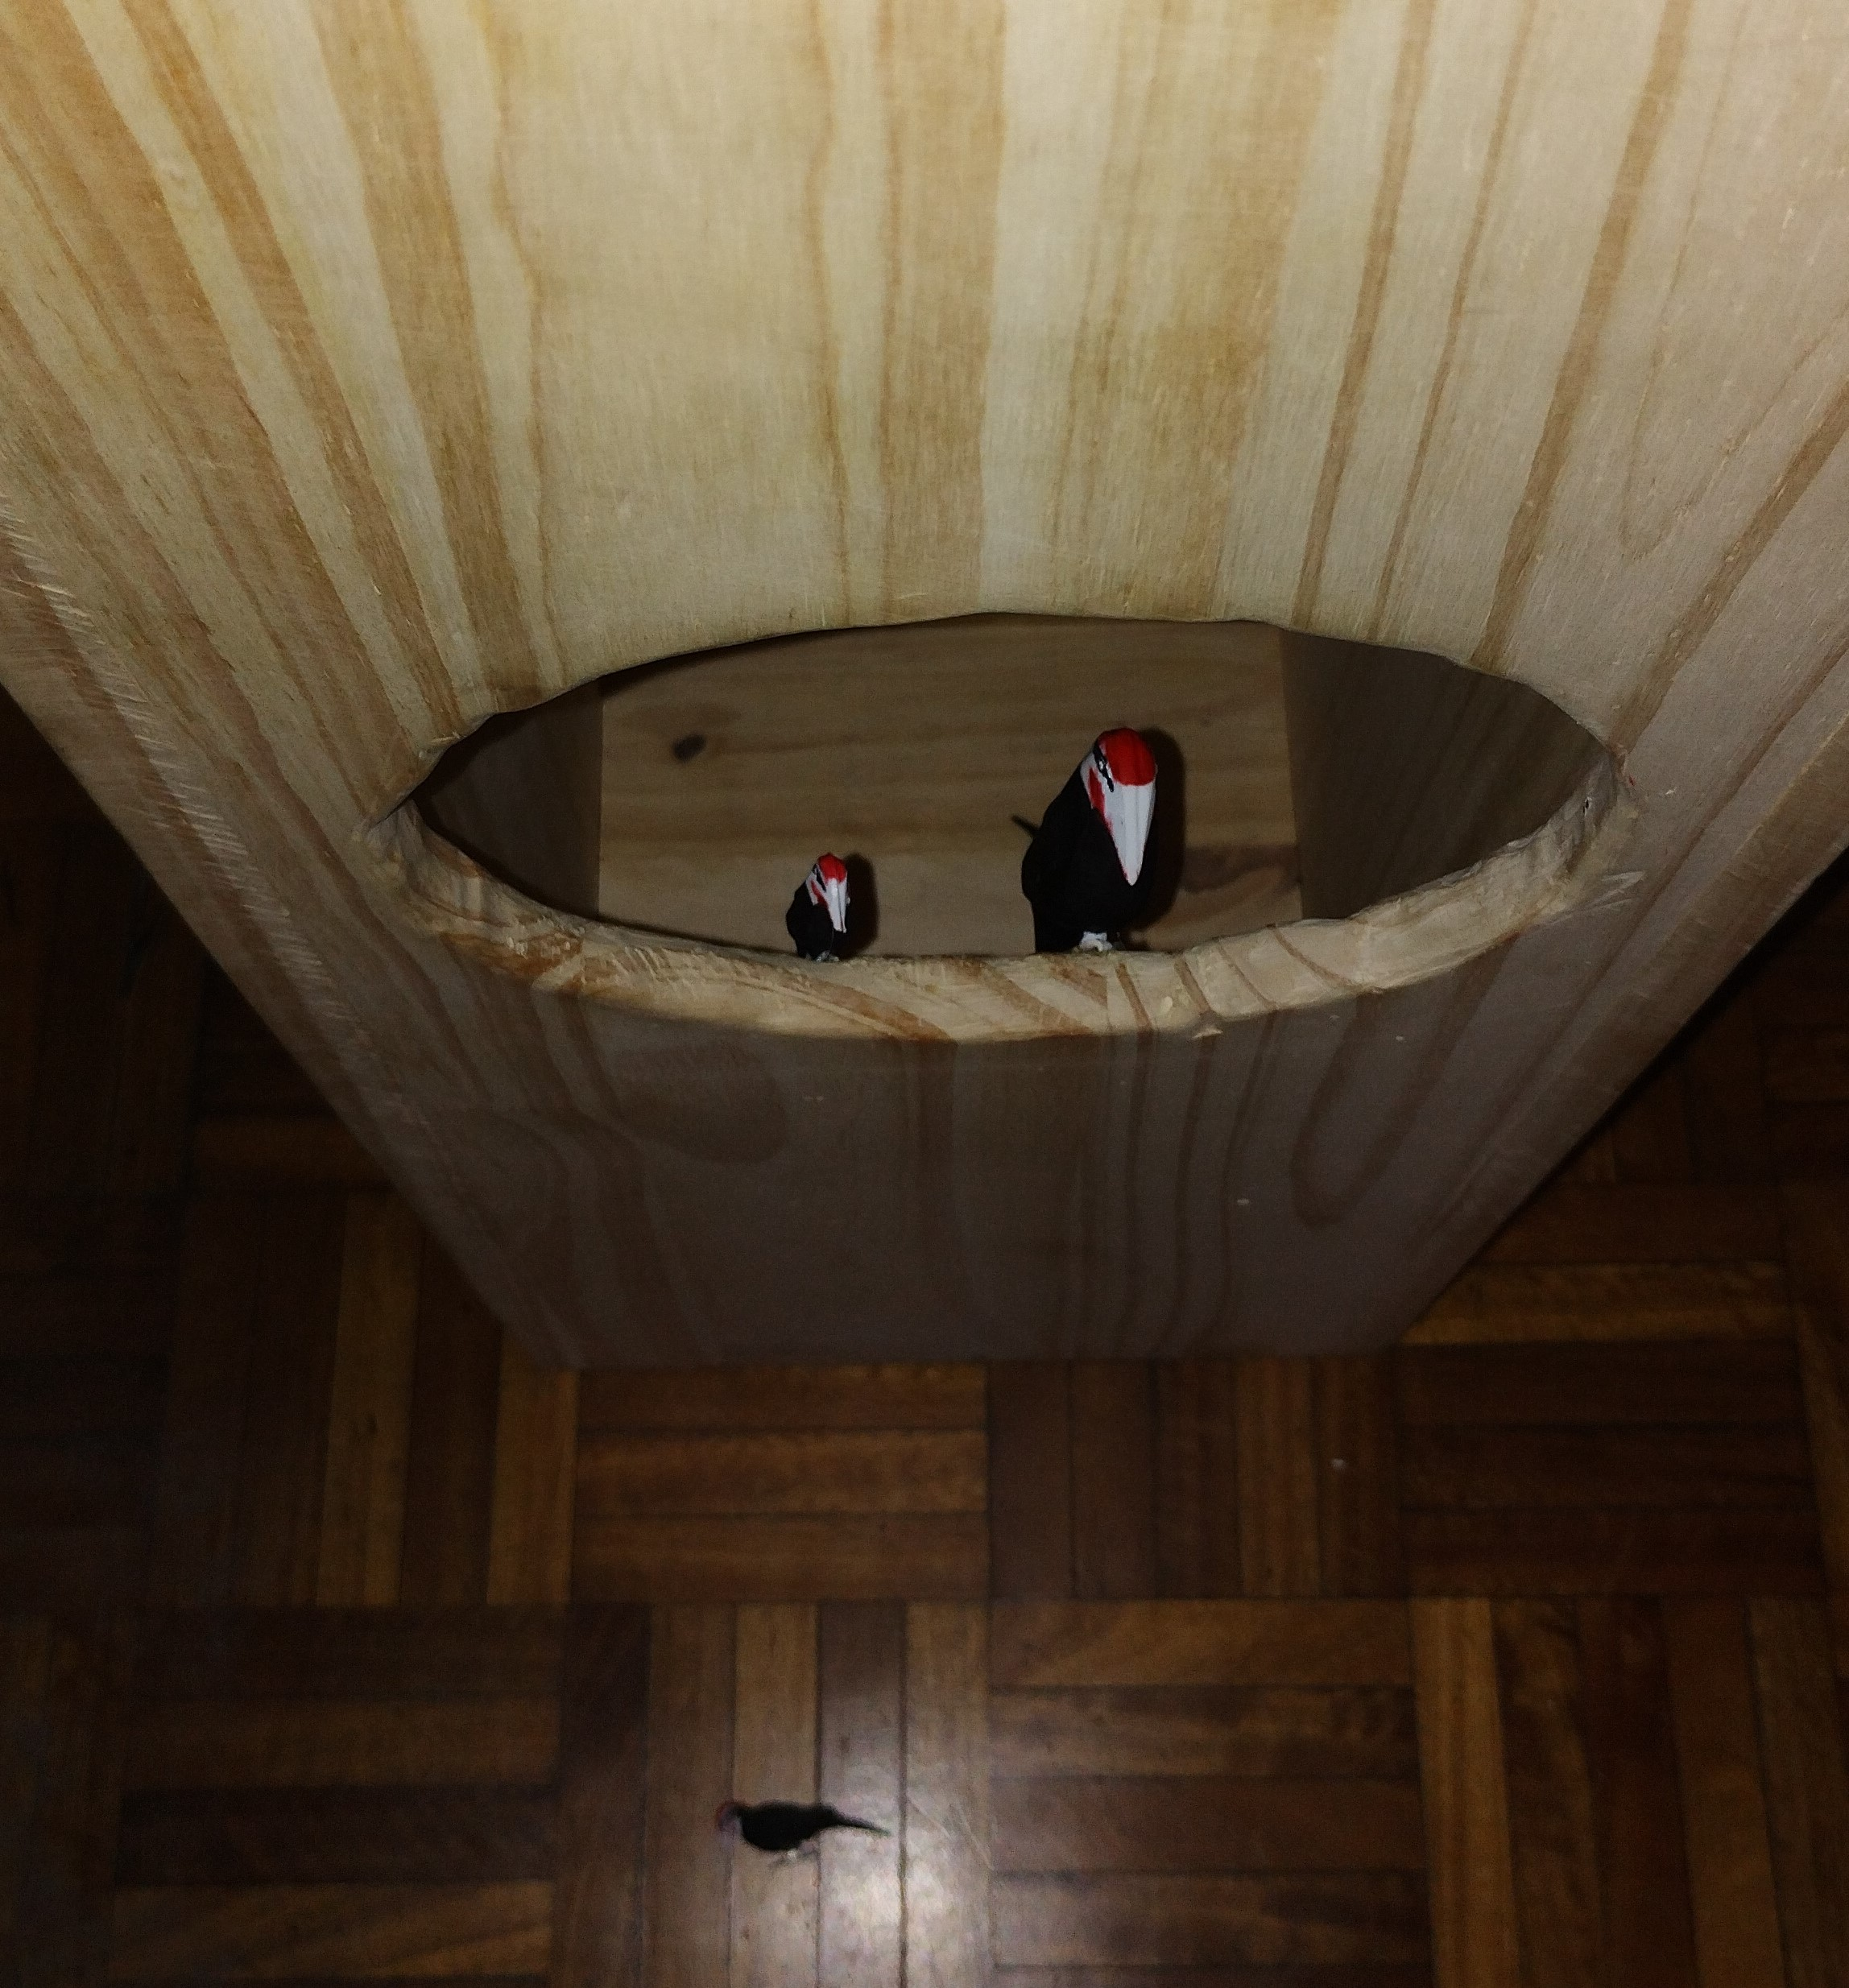
\includegraphics[width=0.5\linewidth]{ImagenesValidacion del prototipo/t-int-fun-04-12-2}
        	\caption{Imagen del exterior del nido en el momento de la trasmisión.}
        \end{subfigure}
	\caption{Validación de funcionalidad \textit{T-INT-FUN-04} y \textit{T-INT-FUN-12}.}
\end{figure}

\Subsection{Validación Pruebas de Comunicación 1}

%El desarrollo de las pruebas de \textit{T-INT-COM2-2} se efectuó sin mayores inconvenientes, logrando la conexión a la distancia necesaria.

\Subsection{Validación Pruebas de Comunicación 2}
Para las pruebas de Comunicación 2 se requiere la computadora de un tercero (biólogo en campo). La primera prueba corresponde a \textit{T-INT-COM02-1} la cual consta en analizar a la capacidad de acceder a los datos del ave guardados en el nido.
\begin{figure}[H]
\centering
	\begin{subfigure}{0.49\textwidth}
		\centering
		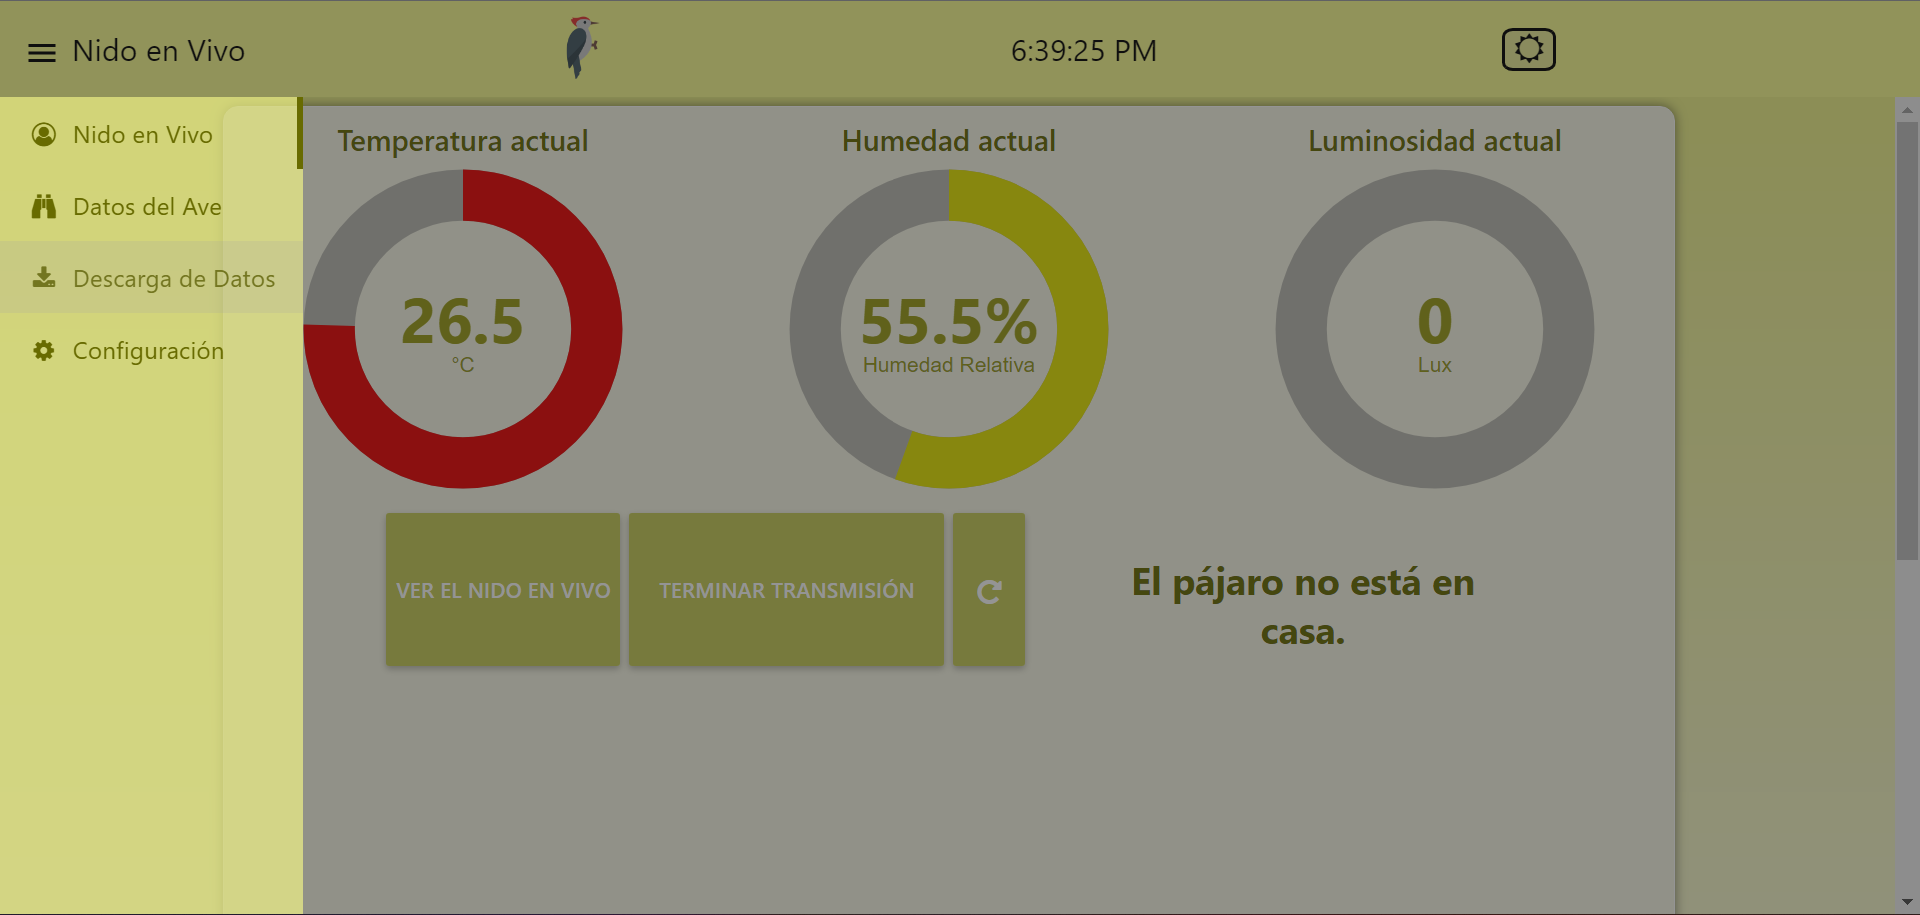
\includegraphics[width=\linewidth]{ImagenesValidacion del prototipo/TINTCOM21a}		
		\caption{Pestaña de descargas.}
	\end{subfigure}\hfill
	\begin{subfigure}{0.49\textwidth}
		\centering
		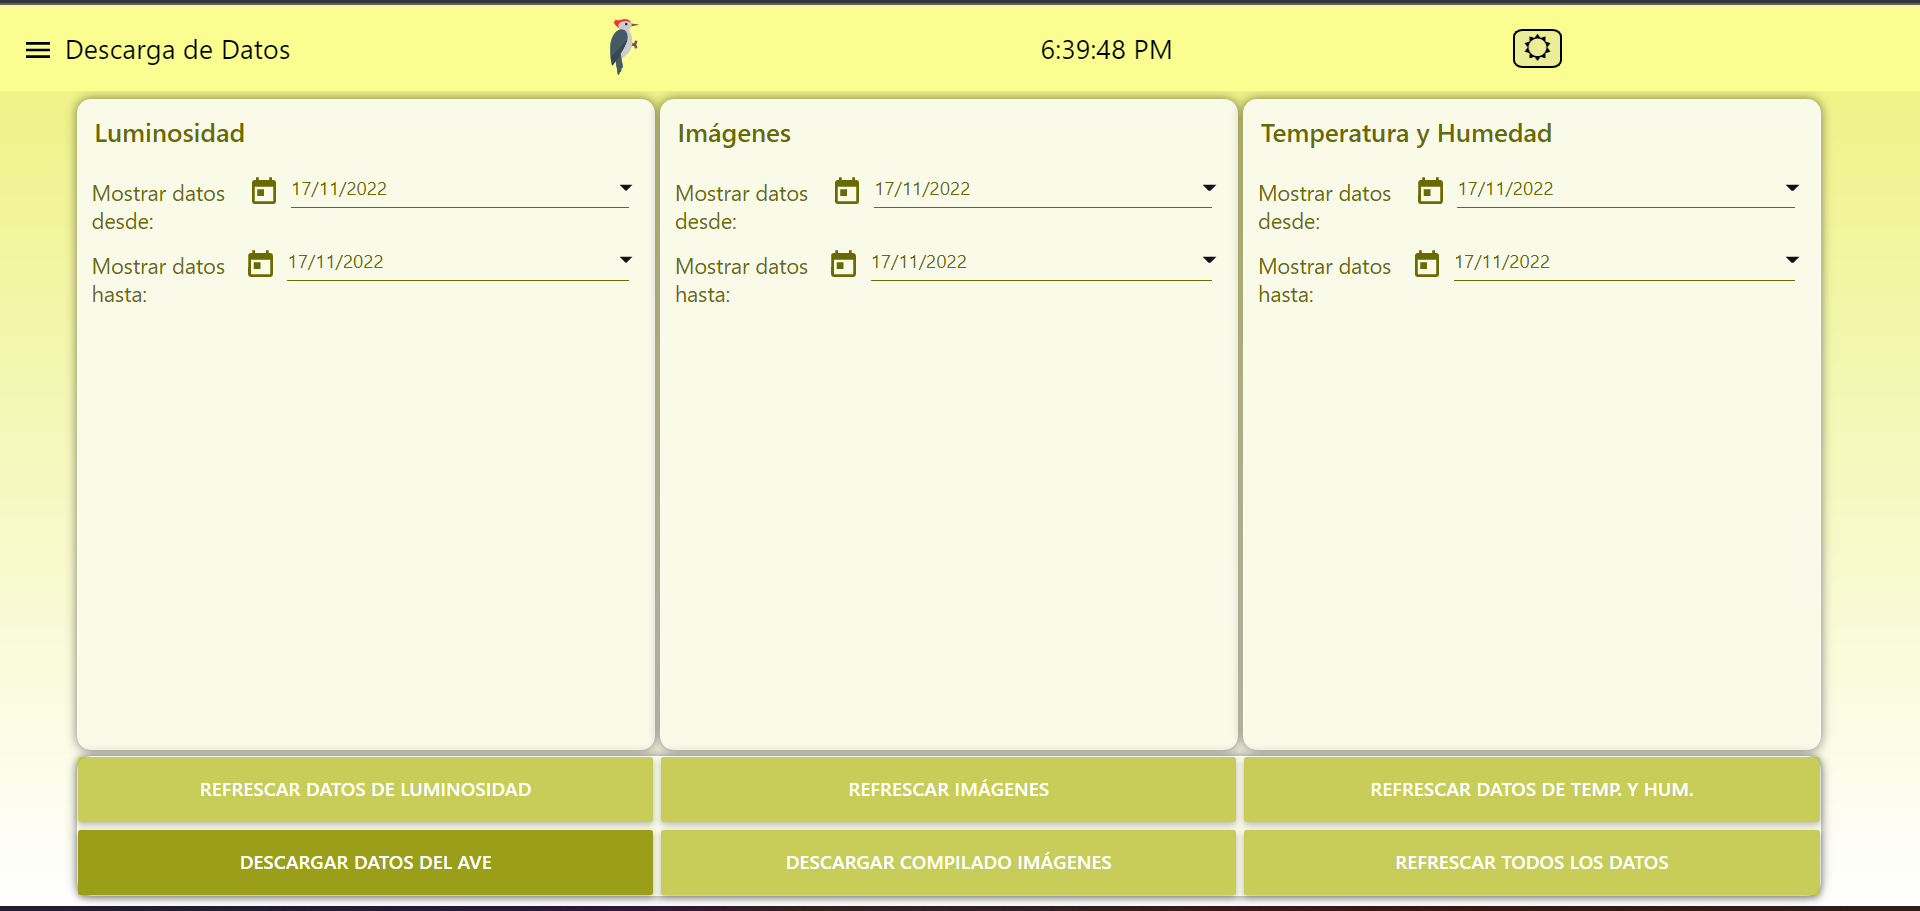
\includegraphics[width=\linewidth]{ImagenesValidacion del prototipo/TINTCOM21b}
		\caption{Botón de descarga.}
	\end{subfigure}
	\caption*{}
\end{figure}
\begin{figure}[H]
	\ContinuedFloat
	\centering
	\begin{subfigure}{\textwidth}
		\centering
		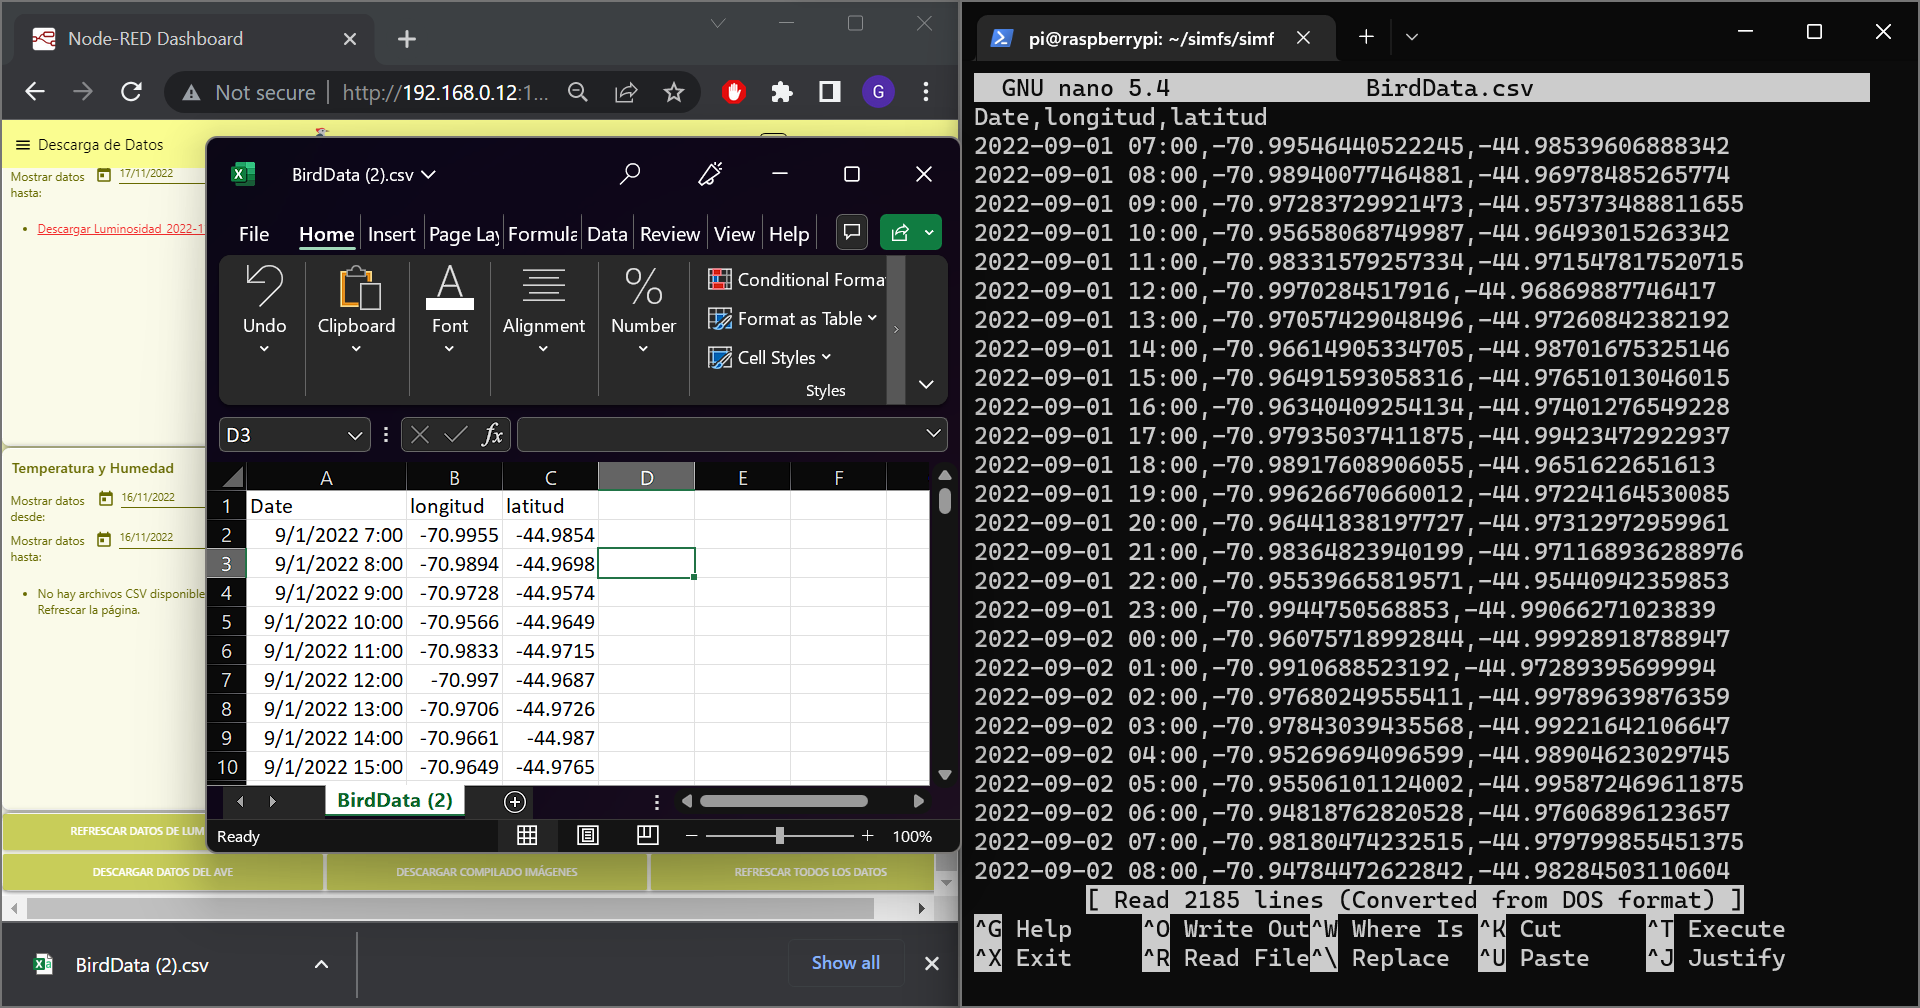
\includegraphics[width=0.8\linewidth]{ImagenesValidacion del prototipo/TINTCOM21}
		\caption{Consola y csv descargado.}
	\end{subfigure}
	\caption{Validación de comunicación \textit{T-INT-COM02-1}.}
\end{figure}

Se observa que los datos descargados que se ven en la izquierda se corresponden con los datos que se encuentran en el nido como se ve a la derecha. Por lo que no hubo una pérdida de datos.
Adicionalmente se utilizó una función de \textit{hash} para comparar los contenidos de ambos archivos y fehacientemente comprobar que son el mismo archivo. 

Se procede a realizar la validación correspondiente a \textit{T-INT-COM02-3}. En esta prueba se de verificar la existencia del archivo \textit{BirdData} luego descargarlo y al acceder nuevamente a la \rspi comprobar que el archivo \textit{BirdData} fue borrado exitosamente.
\begin{figure}[H]
\centering
	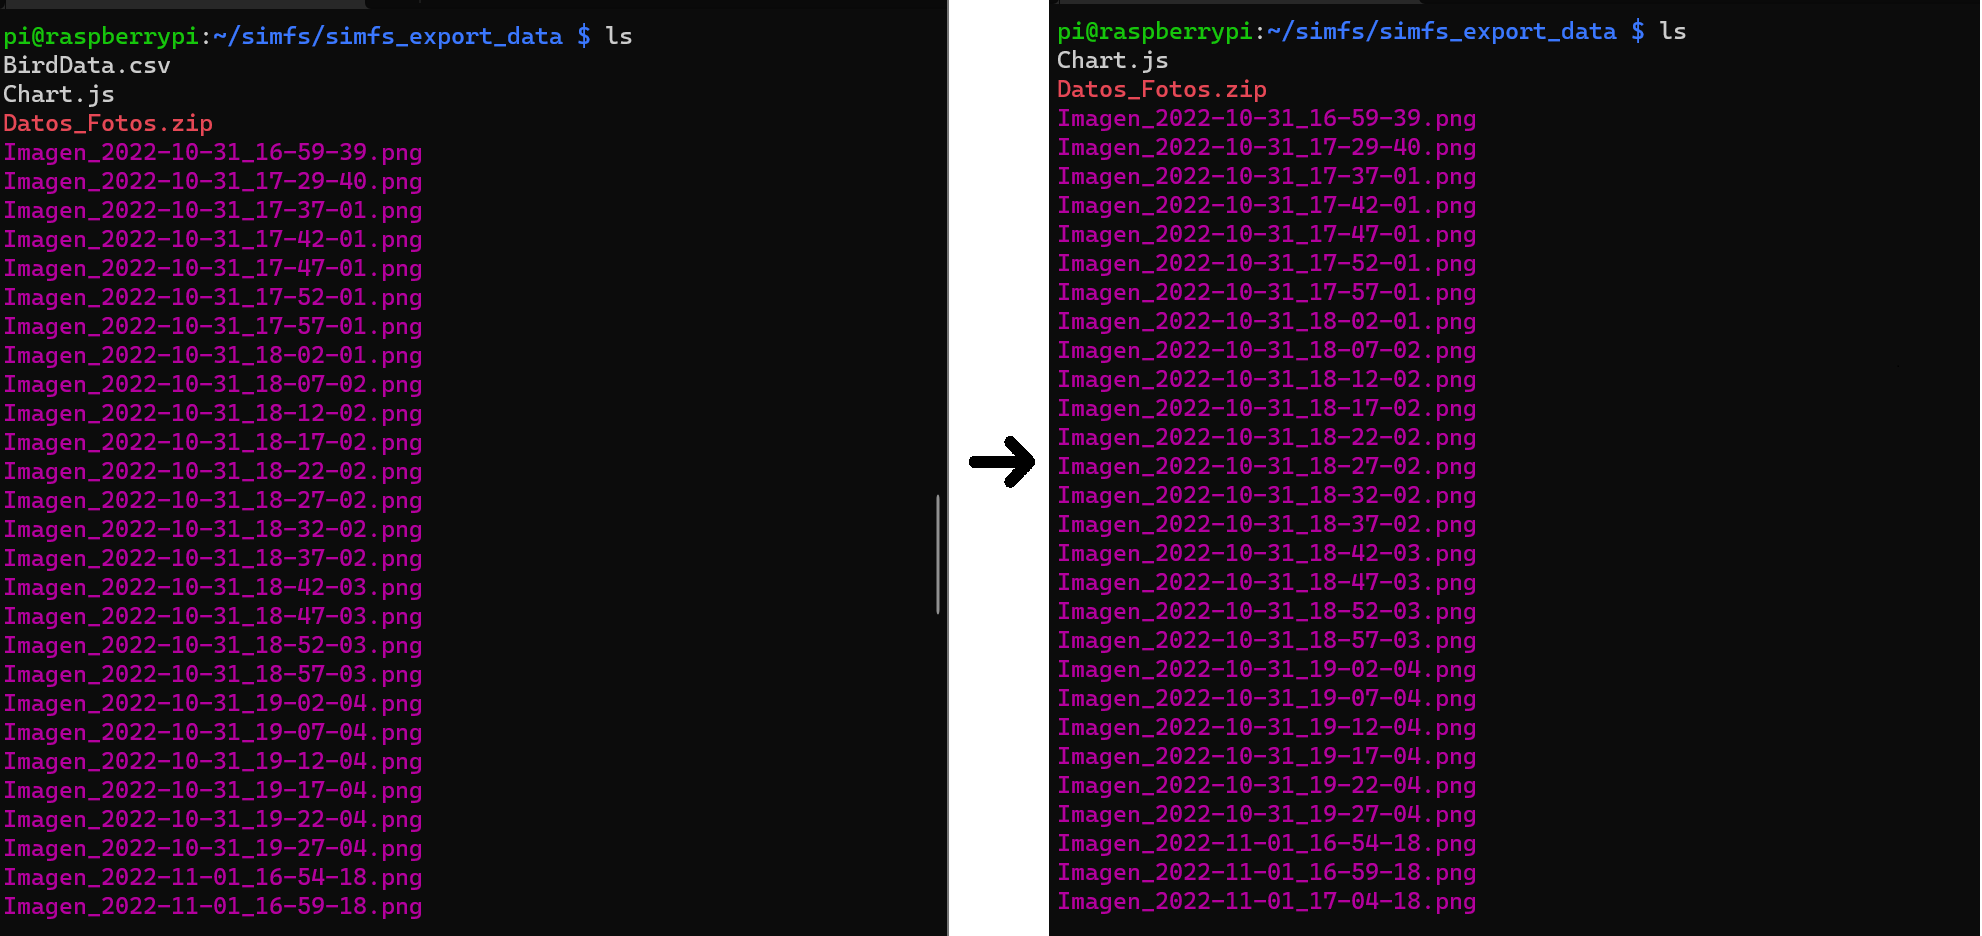
\includegraphics[width=1\linewidth]{ImagenesValidacion del prototipo/TINTCOM23}
	\caption{Validación de comunicación \textit{T-INT-COM02-3}.}
\end{figure}

\Subsection{Validación pruebas de seguridad}

Se dispuso del banco de pruebas \#1 para analizar la aplicabilidad de \textit{T-RAM-SEG-01}. El acceso tanto a la interfaz gráfica del usuario como la del administrador se encuentran restringidas para cualquiera que no posea las credenciales adecuadas.
\begin{figure}[H]
\centering
    	\begin{subfigure}{0.49\textwidth}
        	\centering
        	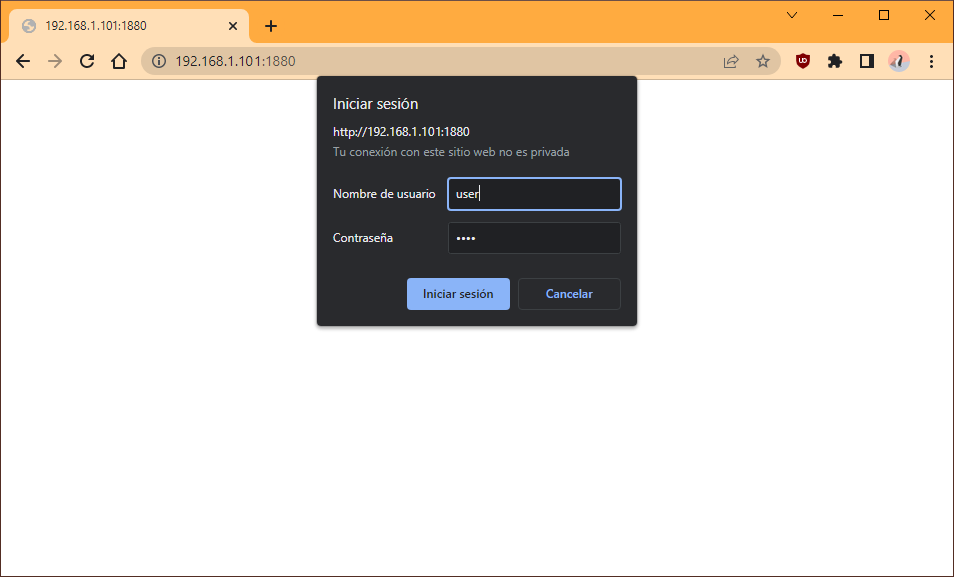
\includegraphics[width=\linewidth]{ImagenesValidacion del prototipo/t-ram-seg-01-1}		
			\caption{Autenticación de usuario para la interfaz gráfica.}
        \end{subfigure}\hfill
        \begin{subfigure}{0.49\textwidth}
        	\centering
        	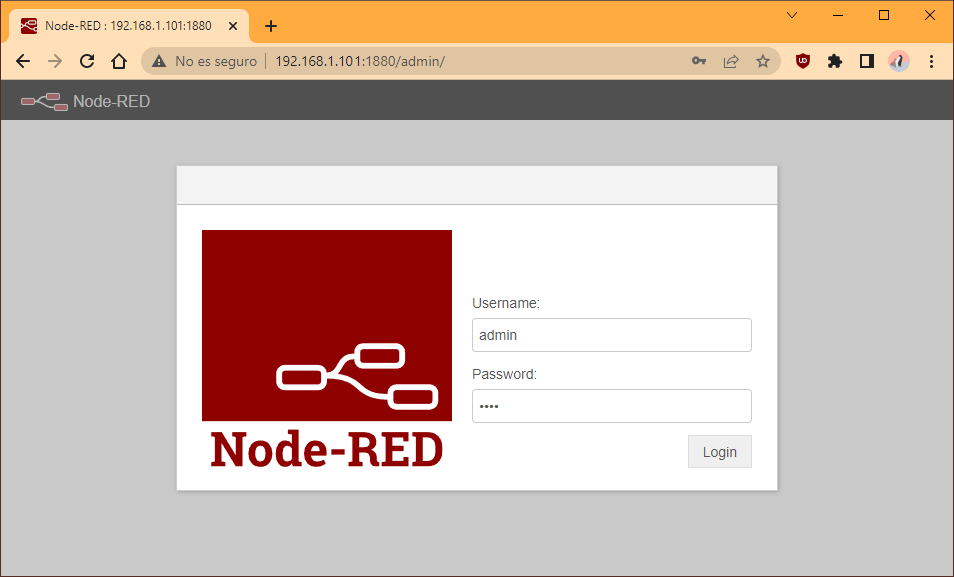
\includegraphics[width=\linewidth]{ImagenesValidacion del prototipo/t-ram-seg-01-2}
        	\caption{Autenticación de administrador para la interfaz gráfica.}
        \end{subfigure}
	\caption{Validación de seguridad \textit{T-RAM-SEG-01}.}
\end{figure}

Se obtuvo un resultado mejor del esperado ya que el hecho de emplear una red WiFi para conectar la unidad del nido con el usuario también requiere del uso de una contraseña. Esto agrega una capa de seguridad extra al sistema.
